% Created:  Thu 10 Jul 2014 04:22 PM
% Modified: Thu 10 Jul 2014 04:22 PM
% @author Josh Wainwright
% File name : quadtree-traversal.tex

\section{Quadtree Traversal}
\label{sec:quadtree_traversal}

Whether the quadtree is stored in memory as a recursive quadtree data
structure, or as hash table, Section~\ref{sub:hash_table_implementation}, the
most important and computationally intensive step is extracting the clusters at
the correct depth and disregarding those data points that can be attributed to
noise.

The quadtree numbering system chosen lends itself very well to analysis based
on spatial location and the proximity of neighbours to a given node being
examined. The neighbours of interest, named \emph{rook's case} neighbours
by~\cite{abel1990comparative}, are the four nodes that lie to the north, east,
sound and west of the current node.

\begin{figure}[tbhp]
	\centering
	\includegraphics[width=0.88\linewidth]{propogation.pdf}
	% TODO caption
	\caption{Propagation}
	\label{fig:propogation}
\end{figure}

When discovering clusters via this propagation technique, care must be taken to
avoid a run-away situation where every node in the tree gets included. This
would happen when looking at the neighbours of a node and blindly including
them. Since every internal node has exactly four neighbours, the propagation
would terminate only when reaching the edge nodes.

Instead, the depth of the node must be considered. Again, the simplest method
is not sufficient. If the propagation is limited to a given node depth, even if
this is not the same as the deepest node, the size of any clusters that are
identified will be limited, as shown in Figure~\ref{fig:propogation-halting}.
Since the depth to consider is not able to change, when the neighbours of the
blue cell are checked, no correct neighbours are found and so the process
terminates. When able to view the larger structure of the cells, however, it is
clear that the structure continues beyond the gap.

\begin{figure}[tbhp]
	\centering
	\includegraphics[width=0.7\linewidth]{propogation-halting.pdf}
	\caption{propogation-Halting}
	\label{fig:propogation-halting}
\end{figure}

To avoid this, a certain amount of leniency must be given when deciding what
constitutes a neighbour. Given an appropriate value, this would allow both of
the larger white cells in Figure~\ref{fig:propogation-halting} to be included.

The \emph{depth range} shall define the levels that are to be considered when
choosing neighbours with respect to a target depth. Since clusters are being
considered areas of increased density of points, all cells with a depth greater
than the target depth shall be allowed, so the purple cells in
Figure~\ref{fig:propogation-halting} would be included when the target depth is
the same as the depth of the included red cells. A depth range of zero is
eqivalent to the situation above where only cells of a given depth are
considered. A depth range of 1 would mean that the white square in
Figure~\ref{fig:propogation-levels}\,b) would be included but not in~c),
whereas a depth range of three would include both.

\begin{figure}[tbhp]
	\centering
	\includegraphics[width=0.88\linewidth]{propogation-levels.pdf}
	\caption{propogation-Levels}
	\label{fig:propogation-levels}
\end{figure}

\begin{figure}[tbhp]
	\centering
	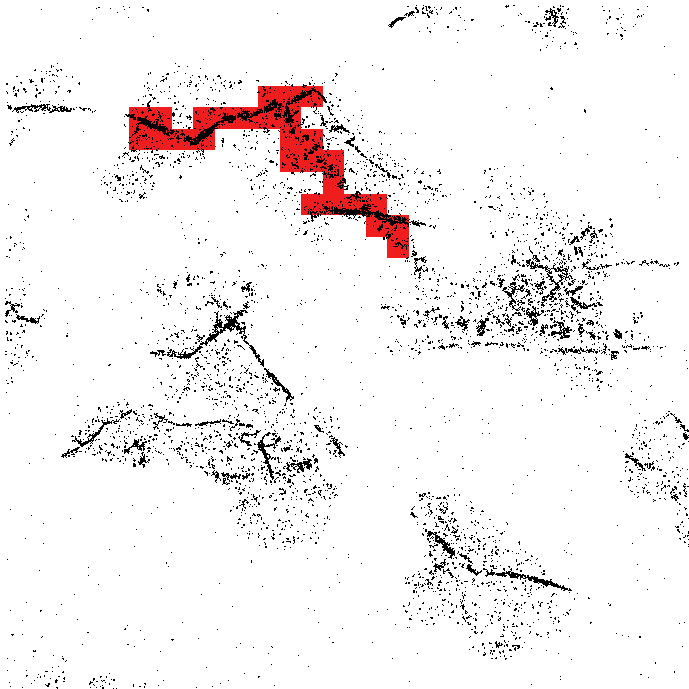
\includegraphics[width=0.88\linewidth]{single-cluster.png}
	\caption{single-Cluster}
	\label{fig:single-cluster}
\end{figure}
